\documentclass[12pt]{report}
\usepackage[utf8]{inputenc}
\usepackage[russian]{babel}
\usepackage{setspace} % для междустрочного интервала
\onehalfspacing % 1.5 интервал между строками

\usepackage{graphicx}
\graphicspath{{pictures/}}

\usepackage[left=30mm, top=20mm, right=20mm, bottom=20mm, nohead, footskip=7mm]{geometry}


\usepackage{listings}

\lstset{
language = python,
extendedchars=\true,
basicstyle=\small\sffamily,
numbers=left,
numberstyle=\tiny,
stepnumber=1,
numbersep=5pt,
showspaces=false,            % показывать или нет пробелы специальными отступами
showstringspaces=false,
showtabs=false,
frame=single,
tabsize=2,
captionpos=t,
breaklines=true,
breakatwhitespace=false,
escapeinside={\#*}{*)},
keepspaces=true
}

\usepackage{multirow} % таблица

\usepackage{titlesec, blindtext, color} 
\definecolor{gray75}{gray}{0.75}
\newcommand{\hsp}{\hspace{20pt}}
\titleformat{\chapter}[hang]{\Large\bfseries}{\thechapter{. }}{0pt}{\Large\bfseries}
\titlespacing{\chapter}{0pt}{-30pt}{12pt} % отступ заголовка сверху
\titleformat{\section}[hang]{\large\bfseries}{\thesection{. }}{0pt}{\large\bfseries}


\begin{document}

\begin{center}
	\begin{spacing}{1}
		\hfill \break
		\footnotesize\textbf{Министерство науки и высшего образования Российской Федерации \\
			Федеральное государственное бюджетное образовательное учреждение \\
			высшего образования\\
			«Московский государственный технический университет\\
			имени Н.Э. Баумана\\
			(национальный исследовательский университет)»\\
			(МГТУ им. Н.Э. Баумана)}\\
		\underline{\noindent\rule{\textwidth}{3pt}}\\
	\end{spacing}
\end{center}

\begin{flushleft}
	ФАКУЛЬТЕТ \underline{{«Информатика и системы управления»}\hspace{6.2cm}}\\
	КАФЕДРА \underline{{ «Программное обеспечение ЭВМ и информационные технологии»}\hspace{1.6cm}}
\end{flushleft}
\hfill \break
\hfill \break
\begin{center}
	\footnotesize\textbf{\large Отчет}\\
	\large{о лабораторной работе \\по дисциплине Анализ Алгоритмов №1\\
	на тему <<Расстояния Левенштейна и Дамерау-Левенштейна>>} 
\end{center}
\hfill \break
\hfill \break
\hfill \break
\hfill \break
\hfill \break
\hfill \break
\hfill \break
\textbf {Студент } 
\textbf{\underline{Брянская Е.В.\hspace{2cm}}}\\
\hfill \break
\textbf {Группа } 
\textbf{\underline{ИУ7-52Б\hspace{3.3cm}}}\\
\hfill \break
\textbf {Преподаватель } \textbf{\underline{Волкова Л.Л.\hspace{0.7cm}}}\\
\hfill \break
\hfill \break
\begin{center} Москва \\2020 \end{center}
\thispagestyle{empty} % выключаем отображение номера для этой страницы


\tableofcontents

\newpage
\chapter*{Введение}
\addcontentsline{toc}{chapter}{Введение}

\textbf{Расстояние Левенштейна}  (рациональное расстояние) – это минимальное количество редакторских операций, которые необходимы для превращения одной строки в другую. 

Под редакторскими операциями подразумеваются:
\begin{itemize}
\item вставка (обозначается, как I - insert);
\item замена (R - replace);
\item удаление (D - delete);
\item также сюда относится совпадение (M - match).
\end{itemize}

Расстояние Левенштейна имеет широкий спектр применения, например, используется в поисковых строках, в программах, отвечающих за автоисправление, автозамену. Помимо этого, оно также применяется в биоинформатике (строение белков представляется строками, состоящими из букв ограниченного алфавита, таким образом, упрощается их анализ).

Существует много алгоритмов, рассчитывающих расстояние Левенштейна, а также их модификаций, которые и будут рассмотрены далее.


\chapter{Аналитическая часть}
\textbf{Цель} данной работы – реализовать и сравнить алгоритмы поиска расстояний Левенштейна и Дамерау-Левенштейна.\\

Для достижения поставленной цели необходимо решить ряд следующих \textbf{задач}:
\begin{enumerate}
\item дать математическое описание расстояний;
\item описать алгоритмы поиска расстояний;
\item оценить затрачиваемую алгоритмами память;
\item реализовать эти алгоритмы ;
\item провести замеры процессорного времени работы алгоритмов на материале серии экспериментов;
\item провести сравнительный анализ алгоритмов.
\end{enumerate}

Поиск расстояния Левенштейна можно описать разными алгоритмами:
\begin{itemize}
\item матричный расчёт;
\item рекурсивный расчёт по формуле;
\item рекурсивный алгоритм, заполняющий незаполненные клетки матрицы.
\end{itemize}

Пусть S1 и S2 – строки длиной N и M соответственно. Тогда расстояние Левенштейна можно рассчитать по следующей рекуррентной формуле:

\begin{equation}
D(i,j) = \left\{ \begin{array}{ll}
 j, & \textrm{$\mbox{если }i = 0$}\\
 i, & \textrm{$\mbox{если }j = 0, i > 0$}\\
min(D(S1[1..i], S2[1.. j - 1])+1,\\
\qquad D(S1[1..i - 1], S2[1..j]) + 1, &\textrm{$\mbox{если }i>0, j>0$}\\
\qquad D(S1[1..i - 1], S2[1..j - 1]) + \\
\qquad+\left[ 
	\begin{array}{ccc}
	0, & \textrm{$\mbox{если }S1[i] == S2[j],)$}\\
	1, & \textrm{иначе}
	\end{array} 
\right.
  \end{array} \right.
\end{equation}

При таком способе расчёта расстояния нужно использовать матрицу размера Len(S1) + 1 x Len(S2) + 1, элементы которого рассчитываются по формуле выше.\\

Что касается \textbf{рекурсивного расчёта}, то возникает проблема большого количества повторных вычислений. Это очень сильно влияет как на время выполнения, так и на занимаемую память.\\

\textbf{Рекурсивный алгоритм, заполняющий незаполненные клетки матрицы,} работает по аналогии с бесконечностями в алгоритме Дейкстры поиска расстояний в графе.\\

\textbf{Расстояние Дамерау-Левенштейна} дополнительно включает операцию перестановки двух соседних символов (транспозицию) и формула выглядит следующим образом:

\begin{equation}
	D(i,j) = \left\{ \begin{array}{ll}
		j, & \textrm{$\mbox{если }i = 0$}\\
		i, & \textrm{$\mbox{если }j = 0, i > 1$}\\ %6554546
		min(D(S1[1..i], S2[1.. j - 1]) + 1,\\
		\qquad D(S1[1..i - 1], S2[1..j]) + 1,\\
		\qquad D(S1[1..i - 1], S2[1..j - 1]) + \\
		\qquad+\left[ 
		\begin{array}{ccc}
			0, & \textrm{$\mbox{если }S1[i] == S2[j],$}\\
			1, & \textrm{иначе}
		\end{array} 
		\right.\\
		\qquad D(S1[1..i], S2[1..j]) + 1), & \textrm{$\mbox{если }i > 1, j > 1,$}\\
		& \textrm{$S1[i] == S2[j - 1],$}\\
		& \textrm{$S1[i - 1] == S2[j]$}\\
		min(D(S1[1..i], S2[1..j - 1]) + 1,\\
		\qquad D(S1[1..i - 1], S2[1..j]) + 1, \\
		\qquad D(S1[1..i - 1], S2[1..j - 1]) + \\
		\qquad+\left[ 
		\begin{array}{ccc}
			0, & \textrm{$\mbox{если }S1[i] == S2[j],$}\\
			1, & \textrm{иначе}
		\end{array} 
		\right.), &\textrm{$\mbox{если }i>0, j>0$}
	\end{array} \right.
\end{equation}

\chapter{Конструкторская часть}

Рассмотрим алгоритмы поиска расстояния Левенштейна и Дамерау-Левенштейна для строк S1, S2, каждая из которых имеет длину N и M соответственно.

\section{Расстояние Левенштейна, матричный алгоритм}
\qquadВ основе этого алгоритма лежит формула (1.2). \\

Задаётся матрица размером (N + 1)x(M + 1). Отдельно обрабатывается тривиальный случай: первая строка и первый столбец. 
Далее компоненты матрицы заполняются по формуле так, что выбирается ход с наименьшей стоимостью. 
Попасть в очередную клетку матрицы можно из левой, верхней и диагональной клеток.\\

Результат вычисления будет находится в ячейке [N - 1][M - 1] (то есть в самом углу справа снизу).\\

\textbf{Схема} алгоритма представлена на Рис. 2.1.

\begin{figure}[h]
	\begin{center}
		{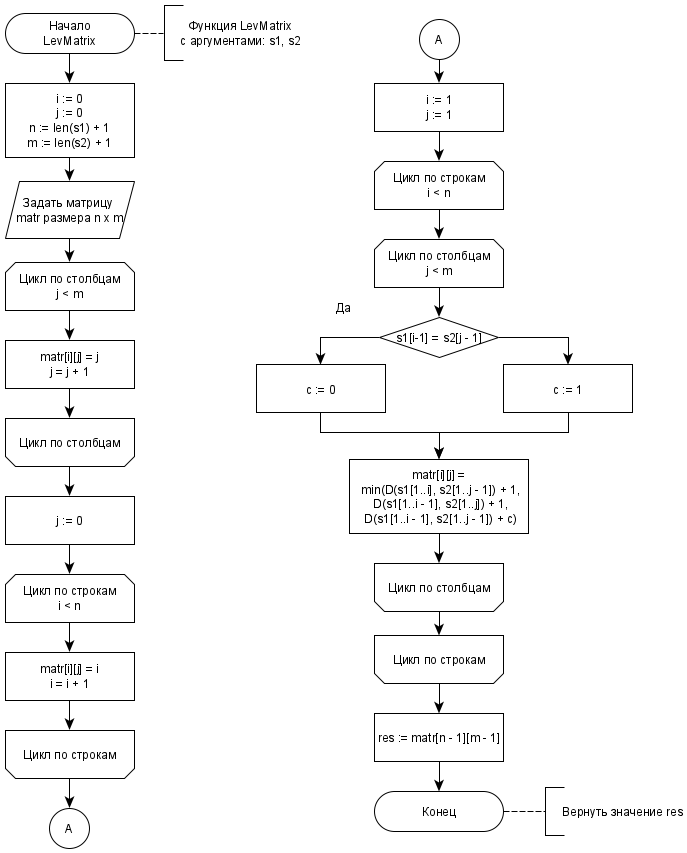
\includegraphics[scale = 1]{LevMatrix}}
		\caption{Матричный алгоритм нахождения расстояния Левенштейна}
	\end{center}
\end{figure}

\section{Расстояние Левенштейна, рекурсивный алгоритм}
\qquadЭтот алгоритм использует рекурсивную формулу для вычисления наименьшего расстояния. \\

На вход подаётся две строки и длины обрабатываемых подстрок i, j, которые в последующем будут рекурсивно изменяться, то есть, (i, j - 1), (i - 1, j - 1), (i - 1, j), до тех пор, пока хотя бы одна из строк не обработается полностью (длина подстроки станет равна нулю). \\

И по завершению работы алгоритмы выбирается наименьшее из трёх полученных значений. \\

\textbf{Схема} алгоритма представлена на Рис. 2.2.

\begin{figure}[h]
	\begin{center}
		{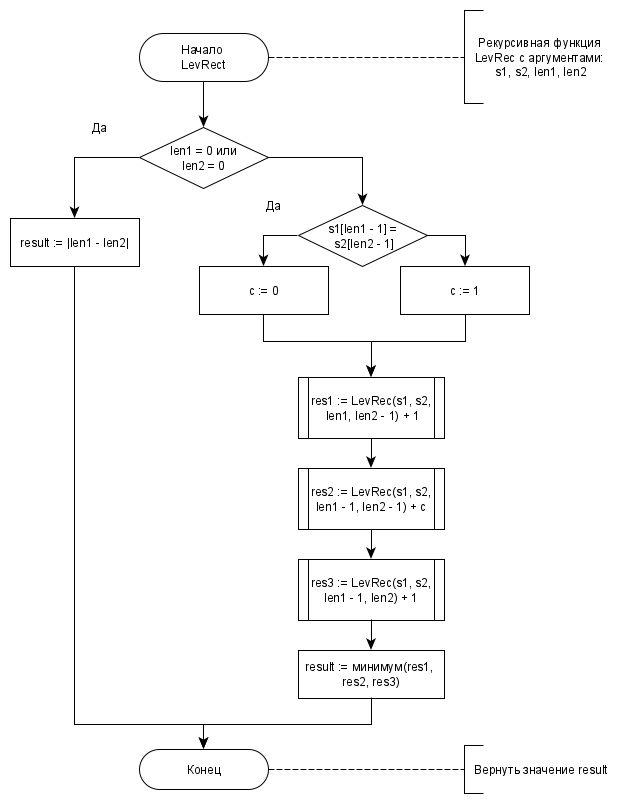
\includegraphics[scale = 0.75]{LevRec}}
		\caption{Рекурсивный расчёт}
	\end{center}
\end{figure}

\section{Расстояние Левенштейна, рекурсивный метод с заполнением матрицы}
\qquadПринцип работы этого алгоритма схож с алгоритмом Дейкстры поиска расстояний в графе. \\

Сначала задаётся матрица размером (N + 1)x(M + 1), все её ячейки заполняются значением +{$\infty$}. Элемент [0][0] заполняется 0, с него и будет начинаться работы алгоритма.\\

На вход рекурсивной функции подаётся матрица, индексы i, j, задающие текущее положение и обрабатываемые строки. По ходу выполнения функции делается выбор, в какую следующую клетку стоит перейти из рассматриваемого ([i][j]). Выбор осуществляется так же, как это было в предыдущих алгоритмов: рассматривается три ячейки с индексами [i + 1][j + 1], [i][j + 1], [i + 1][j] и выбирается та, при переходе из которой расстояние будет наименьшим. И уже из неё осуществляется последующий запуск рекурсивной функции. Важно делать дополнительную проверку на то, чтобы соседняя клетка находилась в пределах матрицы.\\

Результат вычисления будет находится в ячейке [N - 1][M - 1] (то есть в самом углу справа снизу).\\

\textbf{Схема} алгоритма представлена на Рис. 2.3.

\begin{figure}[h]
	\begin{center}
		{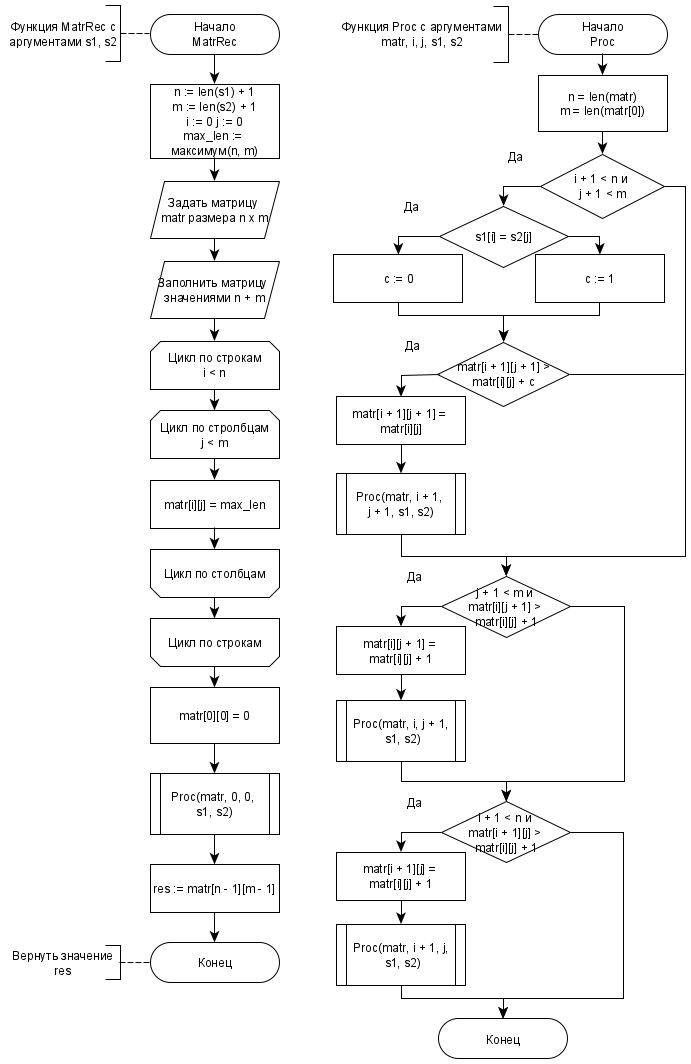
\includegraphics[scale = 0.61]{MatrRec_part2}}
		\caption{Алгоритм, использующий рекурсию и матрицу}
	\end{center}
\end{figure}

\section{Расстояние Дамерау-Левенштейна}
\qquadВ основе алгоритма лежит формула (1.2). В отличие от предыдущих этот метод нахождения минимального расстояния дополнительно учитывает операцию перестановки двух соседних символов. Такая операция называется \textit{транспозицией}\\

Так как этот алгоритм является модификацией описанного выше метода поиска расстояния Левенштейна, то принцип его работы аналогичен. Также создаётся матрица, отдельно отрабатываются тривиальные случаи, выбирается ход с наименьшей стоимостью, только дополнительно проверяется возможность транспозиции.

Результат также будет находится в ячейке [N - 1][M - 1].\\

\textbf{Схема} алгоритма представлена на Рис. 2.4.

\begin{figure}[h]
	\begin{center}
		{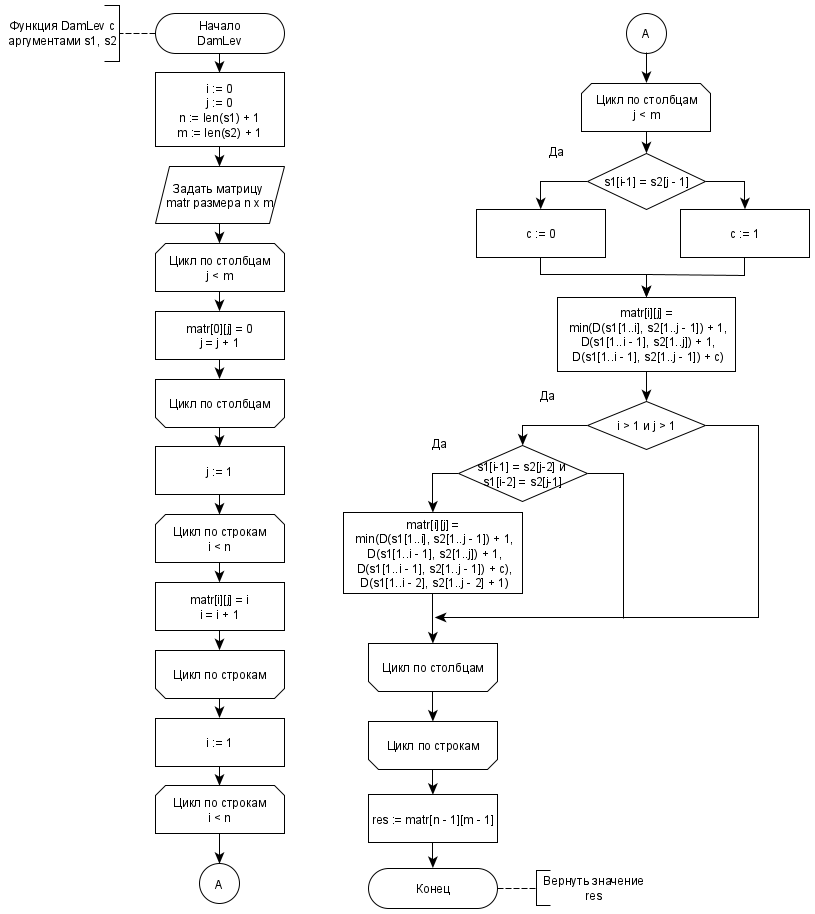
\includegraphics[scale = 0.63]{DanLev}}
		\caption{Алгоритм нахождения расстояния Дамерау-Левенштейна}
	\end{center}
\end{figure}

\section{Требования к ПО}
Для корректной работы алгоритмов и проведения тестов необходимо сделать следующее.
\begin{enumerate}
	\itemОбеспечить возможность ввода двух строк через консоль и выбора алгоритма для расчёта минимального расстояния.
	\itemПрограмма должна рассчитать искомое значение и вывести его на экран, также, если в выбранном методе используется матрица, нужно вывести и её.
	\itemРеализовать функцию замера процессорного времени, которое выбранный метод затрачивает на вычисление результата. Дать возможность пользователю ввести длины рассматриваемых строк через консоль. Вывести результаты замеров на экран.
	\end{enumerate}

\section{Заготовки тестов}
При проверке на корректность работы реализованных функций необходимо провести следующие тесты:
\begin{enumerate}
	\itemобе строки пустые;
	\itemтолько одна из строк пустая;
	\itemполностью совпадающие строки;
	\itemэлементарные тесты на 1 расстояние;
	\itemс расстоянием больше, чем 1;
	\itemс возможной транспозицией.
\end{enumerate}

\chapter{Технологическая часть}
\section{Выбранный язык программирования}
Для выполнения этой лабораторной работы был выбран язык программирования Python, так как есть большой навык работы с ним и с подключаемыми библиотеками, которые также использовались для проведения замеров.
\section{Листинг кода}
\begin{lstlisting}[label=some-code, caption = Матричный алгоритм нахождения расстояния Левенштейна]
def LevMatrix(s1, s2):
	n = len(s1) + 1
	m = len(s2) + 1
	
	matrix = [[i + j for j in range(m)] for i in range(n)]
	
	for i in range(1, n):
		for j in range(1, m):
			const = 0 if (s1[i - 1] == s2[j - 1]) else 1
	
			matrix[i][j] = min(matrix[i][j - 1] + 1,
							   				 matrix[i - 1][j] + 1,
		 	  				   			 matrix[i - 1][j - 1] + const)
	
	return matrix[n - 1][m - 1]
	
	\end{lstlisting}

\begin{lstlisting}[label=some-code, caption = Расстояние Левенштейна - рекурсивный расчёт по формуле]
def LevRecursion(s1, s2, len1, len2):
	if len1 == 0 or len2 == 0:
		return abs(len1 - len2)
	
	const = 0 if (s1[len1 - 1] == s2[len2 - 1]) else 1
	return min(LevRecursion(s1, s2, len1, len2 - 1) + 1,
			   	   LevRecursion(s1, s2, len1 - 1, len2 - 1) + const,
			   		 LevRecursion(s1, s2, len1 - 1, len2) + 1)
			   
def LevRecursion(s1, s2):
	return LevRecursion_process(s1, s2, len(s1), len(s2))
\end{lstlisting}

\begin{lstlisting}[label=some-code, caption = Расстояние Левенштейна - алгоритм с рекурсией и матрицей]
def LevMatrixRecursion_process(matrix, i, j, s1, s2):
	if i + 1 < len(matrix) and j + 1 < len(matrix[0]):
		const = 0 if s1[i] == s2[j] else 1
		if matrix[i + 1][j + 1] > matrix[i][j] + const:
			matrix[i + 1][j + 1] = matrix[i][j] + const
			LevMatrixRecursion_process(matrix, i + 1, j + 1, s1, s2)
	
	if j + 1 < len(matrix[0]) and matrix[i][j + 1] > matrix[i][j] + 1:
		matrix[i][j + 1] = matrix[i][j] + 1
		LevMatrixRecursion_process(matrix, i, j + 1, s1, s2)
	
	if i + 1 < len(matrix) and matrix[i + 1][j] > matrix[i][j] + 1:
		matrix[i + 1][j] = matrix[i][j] + 1
		LevMatrixRecursion_process(matrix, i + 1, j, s1, s2)
		
def LevMatrixRecursion(s1, s2):
	n = len(s1) + 1
	m = len(s2) + 1
	max_len = max(n, m)
	
	matrix = [[max_len for j in range(m)] for i in range(n)]
	matrix[0][0] = 0
	
	LevMatrixRecursion_process(matrix, 0, 0, s1, s2)
	
	return matrix[-1][-1]
\end{lstlisting}

\begin{lstlisting}[label=some-code, caption = Расстояние Дамерау-Левенштейна]
def DamLev(s1, s2):
	n = len(s1) + 1
	m = len(s2) + 1
	
	matrix = [[0] * m for i in range(n)]
	
	for j in range(m):
		matrix[0][j] = j
	
	for i in range(n):
		matrix[i][0] = i
	
	for i in range(1, n):
		for j in range(1, m):
			const = 0 if (s1[i - 1] == s2[j - 1]) else 1
			
			matrix[i][j] = min(matrix[i][j - 1] + 1,
												 matrix[i - 1][j] + 1,
												 matrix[i - 1][j - 1] + const)
			
			if i > 1 and j > 1:
				if s1[i - 1] == s2[j - 2] and s2[j - 1] == s1[i - 2]:
					matrix[i][j] = min(matrix[i][j - 1] + 1,
														 matrix[i - 1][j] + 1,
														 matrix[i - 1][j - 1] + const,
														 matrix[i - 2][j - 2] + 1)
		
	return matrix[n - 1][m - 1]
\end{lstlisting}

\section{Результаты тестов}
\qquadПри тестировании использовалась специальная библиотека \textbf{unittest}. Заранее были написаны необходимые тесты в соответствии с заготовками, приведёнными выше. Тестирование происходит следующим образомЯ: функция возвращает расчитанное значение, и оно сравнивается с тем, которое заранее было внесено в систему, и выводится соответствующий результат.\\

\textbf{Все тесты выполнены.}\\

Сами тесты представлены ниже (Листинг 3.5).
\begin{lstlisting}[label=some-code, caption = Тесты]
import unittest
import main
	
# General tests for all algorithms
class GeneralTest(unittest.TestCase):
	@unittest.skip("General Tests were skipped")
	
	def setUp(self):
		self.function = None
	
	# Обработка пустых строк
	def test_empty_str(self):
		self.assertEqual(self.function("", ""), 0)
		self.assertEqual(self.function("", "12345"), 5)
		self.assertEqual(self.function("98765", ""), 5)
	
    # Совпадающие строки
	def test_match(self):
		self.assertEqual(self.function("1", "1"), 0)
		self.assertEqual(self.function("12qw", "12qw"), 0)
		self.assertEqual(self.function("AbC", "AbC"), 0)
		self.assertEqual(self.function("Abc", "abc"), 1)
	
	# Простые тесты
	def test_easy(self):
		self.assertEqual(self.function("1", "2"), 1)
		self.assertEqual(self.function("123", "1"), 2)
		self.assertEqual(self.function("1", "123"), 2)
		self.assertEqual(self.function("a", "ab"), 1)
		self.assertEqual(self.function("ab", "a"), 1)
		self.assertEqual(self.function("a5c", "abc"), 1)
	
# Тесты для алгоритма поиска расстояния Левенштейна
class LevTest(GeneralTest):
	def test_lev(self):
		self.assertEqual(self.function("1234", "51437"), 3)
		self.assertEqual(self.function("012343563", "7891234356a"), 4)
		self.assertEqual(self.function("01213425", "671213425"), 2)
		self.assertEqual(self.function("abccde", "cdeabc"), 6)
	
# Тесты для алгоритма поиска расстояния Дамерау-Левенштейна
class DemLevTest(GeneralTest):
	def setUp(self):
		self.function = main.DamLev
	
	# Тесты на поиск транспозиций
	def test_demlev(self):
		self.assertEqual(self.function("qw", "wq"), 1)
		self.assertEqual(self.function("132", "123"), 1)
		self.assertEqual(self.function("1001", "0110"), 2)
		self.assertEqual(self.function("2143", "1234"), 2)
	
# Все алгоритмы поиска расстояния Левенштейна проходят не только общие тесты, но и специально написанные LevTest
	
# Алгоритм поиска расстояния Левенштейна (матричный)
class LevMatrixTest(LevTest):
	def setUp(self):
		self.function = main.LevMatrix
	
# Алгоритм поиска расстояния Левенштейна (рекурсия)
class LevRecursionTest(LevTest):
	def setUp(self):
		self.function = main.LevRecursion

# Алгоритм поиска расстояния Левенштейна (матрица + рекурсия)
class LevMatrixRecursionTest(LevTest):
	def setUp(self):
		self.function = main.LevMatrixRecursion
	
	
# Запуск тестов
if __name__ == "__main__":
	unittest.main()
\end{lstlisting}

\section{Оценка памяти}
\qquadРассчитаем память, максимально затрачиваемую каждым алгоритмом при обработке строк s1 и s2. Для упрощения вычислений примем длины строк равными n.\\

\underline{Расстояние Левенштейна (матрица)}\\

Память в этом алгоритме затрачивается на хранение самой матрицы и двух строк.\\

$M_{matrix} = (n + 1)*(n + 1)*sizeof(int) = (n + 1)^2 * 16 байт$\\

$M_{strings} = 2*n*sizeof(char) = 2*n байт$\\

$M = (n + 1)^2 * 16 + 2*n = 16 * n^2 + 34 * n + 16 байт$\\

\underline{Расстояние Левенштейна (рекурсивный расчёт)}\\

Так как это рекурсивный расчёт, то память используется при каждом вызове функции. Функция принимает на вход 2 строки (по значению) и 2 значения, которые являются размерами строк. Максимальная глубина рекурсии n + n. \\

$M = (n + n) * (2 * n * sizeof(char) + 2 * sizeof(int)) = 2 * n * (2 * n + 2 * 16) = 2 * n * (2 * n + 32) = 4 * n^2 + 64 * n байт$\\
\\

\underline{Расстояние Левенштейна (матрица + рекурсия)}\\

Память в этом алгоритме затрачивается для хранения матрицы и при каждом вызове функции. И максимальная глубина рекурсии n + n.\\

$M_{matrix} = (n + 1)*(n + 1)*sizeof(int) = (n + 1)^2 * 16 байт$\\

$M_{recursion} = (n + n) * (2 * n * sizeof(char) + 2 * sizeof(int)) = 2 * n * (2 * n + 2 * 16) = 2 * n * (2 * n + 32) = 4 * n^2 + 64 * n байт$\\

$M = 16 * n^2 + 32 * n + 16 + 4 * n^2 + 64 * n = 20 * n^2 + 96 * n + 16$\\
\\

\underline{Расстояние Дамерау-Левенштейна (матрица)}\\

Затраты на память такие же, как в матричном методе поиска расстояния Левенштейна.\\

$M = (n + 1)^2 * 16 + 2*n = 16 * n^2 + 34 * n + 16 байт$\\

\newpage\section{Среда и инструменты для замера времени}
\qquadЗамер процессорного времени осуществлялся с помощью специальной библиотеки \textbf{time}. Осуществление замеров указано ниже (Листинг 3.6). \\

При замерах пользователь указывает длину строк (для того, чтобы проще было составить далее сравнительную таблицу, длины строк примем одинаковыми). Далее программно генерируются строки, которые далее будет анализироваться.\\

\begin{lstlisting}[label=some-code, caption = Замеры процессорного времени]
# Generating a random line
def RandomString(number):
	letters = string.ascii_lowercase
	return ''.join(random.choice(letters) for i in range(number))

def MeasureTime(length):
	s1 = RandomString(length)
	s2 = RandomString(length)
	
	print(">>> Generated string 1: ", s1)
	print(">>> Generated string 2: ", s2)
	
	print("\n---Levenshtein distance (matrix)---")
	TestTime(LevMatrix, s1, s2)
	
	print("---Levenshtein distance (recurtion)---")
	TestTime(LevRecursion, s1, s2)
	
	print("---Levenshtein distance (matrix + recurtion)---")
	TestTime(LevMatrixRecursion, s1, s2)
	
	print("---Damerau-Levenshtein distance (matrix)---")
	TestTime(DamLev, s1, s2)
	
\end{lstlisting}

\chapter{Исследовательская часть}
Как было упомянуто выше, для облегчения проведения анализа принимается, что длины обрабатываемых строк равны. $len1 = len2 \in \left\lbrace 3, 6, 10, 15, 20, 40, 70, 100, 300\right\rbrace$. Содержимое строк генерируется случайным образом. \\

Каждый замер проводится 5 раз для получения более точного среднего результата.

\begin{table}[ph]
	\caption{Результаты измерений}
	\centering
	\begin{tabular}{|c|c|c|c|c|c|c|c|c|c|c|}
		\hline
		& 3 & 6 & 10 & 15 & 20 & 40 & 70 & 100 & 300\\
		\hline
		Левенштейн & $7.998*$ & $2.383*$ & $6.208*$ & 0.0002 & 0.0002 & 0.001 & 0.003 & 0.005 & 0.049\\
		(матрица) &$10^{-6}$&$10^{-5}$&$10^{-5}$&&&&&&\\
		\hline
		Левенштейн & $2.69*$ & $0.004$ & $3.587$ &---&---&---&---&---&---\\
		(рекурсия) &$10^{-5}$&&&&&&&&\\
		\hline
		Левенштейн & $1.854*$ & $6.123*$ & $0.0002$ & 0.0004 & 0.0008 & 0.005 & 0.029 & 0.085 & 2.687\\
		(матрица+ &$10^{-5}$&$10^{-5}$&&&&&&&\\
		рекурсия &&&&&&&&&\\
		\hline
		Дамерау- & $9.732*$ & $3.05*$ & $7.658*$ & 0.0002 & 0.0003 & 0.006 & 0.004 & 0.008 & 0.068\\
		Левенштейн &$10^{-6}$&$10^{-5}$&$10^{-5}$&&&&&&\\
		\hline	
	\end{tabular}
\end{table}

Важно отметить, что замеры для рекурсивного алгоритма поиска расстояния Левенштейна не были произведены в ряде случае, так как время рассчёта превышает 7 минут.\\

Согласно полученным данным можно сделать несколько выводов:
\begin{itemize}
	\itemдостаточно ожидаемым результатом стали показатели алгоритма поиска расстояния Левенштейна с использованием рекурсии. При обработке строк, длина которых больше 10, время выполнения резко возрастает и достигает значения в несколько минут;
	\itemсамым быстродейственным оказался матричный метод поиска расстояния Левенштейна;
	\itemалгоритм Дамерау-Левенштейна также достаточно эффективный, лишь немного уступает матричному алгоритму;
	\itemалгоритм поиска расстояния Левенштейна, построенный на рекурсии и матрице, имеет показатели гораздо лучшие, чем у алгоритма, использующего только рекурсию; но уступает другим по быстродействию.
\end{itemize}

\chapter*{Заключение}
\addcontentsline{toc}{chapter}{Заключение}
В ходе лабораторной работы была достигнута поставленная цель, а именно были изучены, реализованы алгоритмы поиска наименьшего расстояния, также произведён сравнительный анализ. \\

В процессе выполнения были решение все задачи. Описаны все рассматриваемые алгоритмы, оценена затрачиваемая память при их реализации, кроме того, были сделаны замеры процессорного времени работы каждого на материале серии экспериментов и сделаны соответствующие выводы.

\end{document}